
% ************************* APPENDICE C - GUIDA ALL'ESPERIMENTO **********************

\chapter{Guida all'esperimento}
\label{appendice3}
% *************************
\section*{Avviare interfaccia grafica}

Se si desidera collegare l’Intel\textsuperscript\textregistered Joule\texttrademark\hspace{1mm}ad uno schermo tramite cavo HDMI, una volta avviato il robot premere \text{Alt+F2} per attivare la shell ed effettuare il login (nome utente e password sono entrambi: "\verb!robot!") poi digitare:

\medskip
\begin{tcolorbox}
\begin{verbatim}
>> ./init.sh
\end{verbatim}
\end{tcolorbox}

Questo chiederà conferma ("\verb!y/n!", inserire "\verb!y!") ed avvierà l'interfaccia grafica.
% *************************
\section*{Connessione al robot da remoto}
Il robot è configurato per generare automaticamente una rete Wi-Fi aperta all'accensione, con nome \verb!rosnet!. Per interagire a distanza, connettersi a questa rete, dopodiché sarà possibile eseguire comandi direttamente sul robot tramite \verb!ssh! come mostrato di seguito.

\medskip
\begin{tcolorbox}
\begin{verbatim}
>> ssh -X robot@10.42.0.1 -p 22
\end{verbatim}
\end{tcolorbox}

Alternativamente è possibile utilizzare l’ambiente \verb!ROS! in locale riferendosi comunque al master che è sul robot  tramite i comandi (da eseguire su ogni shell che si vuole connettere)
\medskip
\begin{tcolorbox}
\begin{verbatim}
>> export ROS_MASTER_URI=http://10.42.0.1:11311
>> export ROS_HOSTNAME=10.42.0.181
\end{verbatim}
\end{tcolorbox}

In questo contesto non bisogna connettersi tramite \verb!ssh!, tuttavia è necessario essere connessi alla rete \verb!rosnet!): ciò permette ad esempio di sfruttare \verb!Rviz! con le risorse del computer che si sta utilizzando, senza dover fare streaming video dalla Intel\textsuperscript\textregistered Joule\texttrademark, metodo molto più lento e poco reattivo.
% *************************
\section*{Autocalibrazione delle UWB}

Le ancore devono essere disposte con il seguente setup (Figura~\ref{fig:uwb_axis}):

\begin{figure}[h] 
\centering    
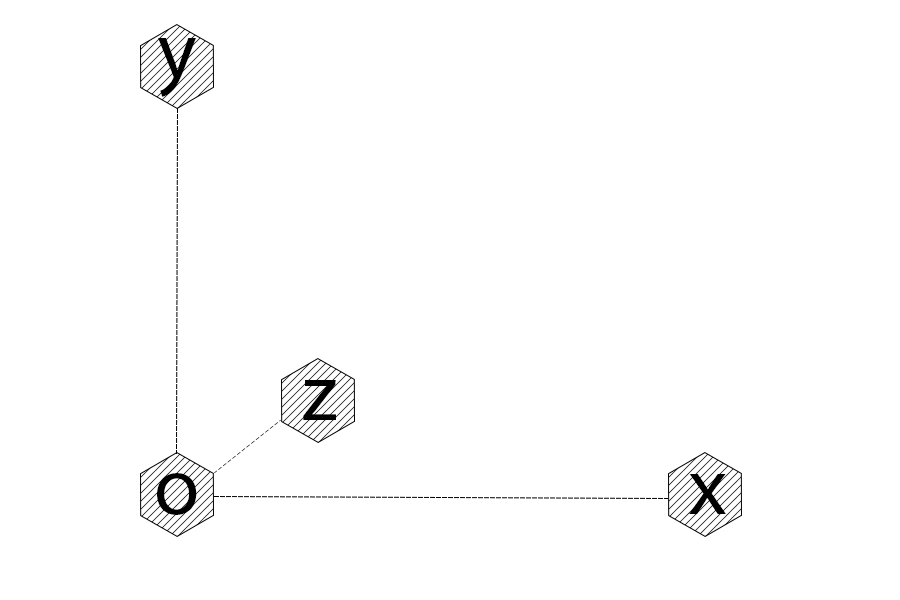
\includegraphics[width=0.45\textwidth]{Appendice3/Fig/uwb_axis.png}
\caption[Assi UWB]{Assi UWB}
\label{fig:uwb_axis}
\end{figure}

Per eseguire l’autocalibrazione basta eseguire il seguente bash script, che si trova nella directory \verb!/home/robot!:

\medskip
\begin{tcolorbox}
\begin{verbatim}
>> cd
>> ./autocalibration.sh
\end{verbatim}
\end{tcolorbox}

Una volta terminata la procedura verranno automaticamente impostate le distanze relative tra le varie ancore e si aprirà un’immagine riassuntiva che mostrerà i risultati dell’autocalibrazione. Alle due domande che appariranno sulla command window rispondere entrambe le volte con \verb!“n”!.
% *************************
\section*{Positioning}

Per avviare il nodo che localizza le due tag poste sul robot:

\medskip
\begin{tcolorbox}
\begin{verbatim}
>> roslaunch charlie_pkg start_uwb.launch
\end{verbatim}
\end{tcolorbox}

Il tag che deve essere posizionato in testa al robot è quello con "\verb!ID = 0x6760!".
Dato che ad ogni accensione l’ordine con cui vengono letti ed interpretati i tag non è sempre lo stesso, all’interno dello script è stato implementata la capacità di leggere l’\verb!ID! delle tag e quindi impostare la tag giusta come testa.
% *************************
\section*{Acquisizione della mappa}

Il robot può essere posizionato in qualsiasi punto dello spazio e con qualsiasi orientazione, non vi è alcuna necessità che gli assi del Lidar (Figura~\ref{fig:lidar_axis}) siano orientati come quelli del setup delle UWB in quanto la posa con cui si inizia ad acquisire la mappa verrà salvata in un file dedicato.

\medskip
\begin{figure}[h] 
\centering    
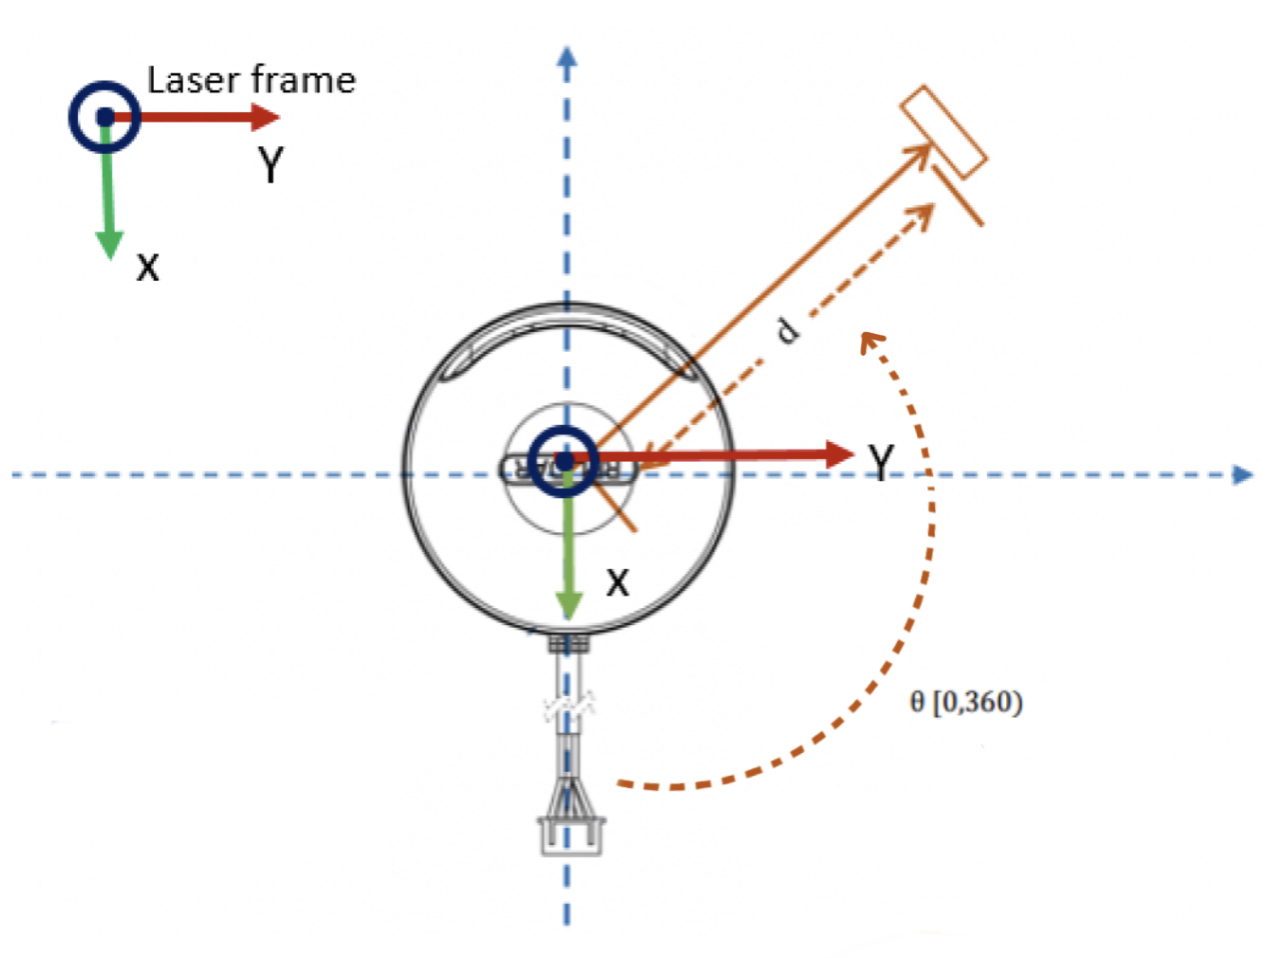
\includegraphics[width=0.6\textwidth]{Appendice3/Fig/lidar_axis.png}
\caption[Assi Lidar]{Assi Lidar}
\label{fig:lidar_axis}
\end{figure}
\medskip

Poiché l’origine della mappa che si andrà ad acquisire corrisponderà al punto in cui viene avviato \verb!hector_slam!, prima di iniziare il processo di mappatura è necessario salvare la distanza relativa tra i sistemi di riferimento di UWB e Lidar e la relativa orientazione. 
Avviare in primis il sistema UWB tramite il comando:

\medskip
\begin{tcolorbox}
\begin{verbatim}
>> roslaunch charlie_pkg start_uwb.launch
\end{verbatim}
\end{tcolorbox}
Appena i dati inizieranno a scorrere sullo schermo, avviare il salvataggio della posa corrente con il comando:

\medskip
\begin{tcolorbox}
\begin{verbatim}
>> roslaunch charlie_pkg save_map_origin.launch
\end{verbatim}
\end{tcolorbox}

Questo avvierà anche la comunicazione seriale, grazie alla quale sarà possibile ricavare l'orientazione del robot rispetto al frame \verb!UWB! (filtrata dal software a bordo dell'STM\textsuperscript\textregistered).

Una volta che la procedura è completata, chiudere la finestra di lavoro. Si consiglia comunque di segnare la posizione e l'heading del punto in questione poiché, a causa del forte rumore presente sul sistema UWB, potrebbe rivelarsi necessario riposizionare il robot e ripetere tale acquisizione.

A questo punto è possibile acquisire una nuova mappa semplicemente digitando:
\medskip
\begin{tcolorbox}
\begin{verbatim}
>> roslaunch charlie_pkg new_map.launch
\end{verbatim}
\end{tcolorbox}

Questo avvierà Lidar, \verb!hector_mapping! e \verb!Rviz! mostrando a schermo lo stato corrente dell'acquisizione della mappa. 
Una volta soddisfatti del risultato ottenuto, posizionarsi nella cartella in cui si desidera salvare la mappa acquisita (tramite il comando \verb!cd!)  e digitare il seguente comando:

\medskip
\begin{tcolorbox}
\begin{verbatim}
>> rosrun map_server map_saver -f nomemappa
\end{verbatim}
\end{tcolorbox}
% *************************
\section*{Localizzazione e navigazione}

Nel launch file localization.launch inserire il percorso della mappa che si desidera utilizzare e avviare il sistema con i seguenti comandi:

\medskip
\begin{tcolorbox}
\begin{verbatim}
>> roslaunch charlie_pkg start_uwb.launch
>> roslaunch charlie_pkg localization.launch
\end{verbatim}
\end{tcolorbox}

Si aprirà una istanza di \verb!Rviz! slla quale verrà mostrata la posa stimata del robot e su cui sarà possibile indicare un goal tramite il comando \verb!2DNavgoal!.
Per attivare i motori e permettere al robot di spostarsi, pubblicare il seguente messaggio sul topic \verb!start_and_stop!:

\medskip
\begin{tcolorbox}
\begin{verbatim}
>> rostopic pub /start_and_stop std_msgs/Float64 "data: 1.0"
\end{verbatim}
\end{tcolorbox}

Per fermare i motori in qualsiasi momento:

\medskip
\begin{tcolorbox}
\begin{verbatim}
>> rostopic pub /start_and_stop std_msgs/Float64 "data: 0.0"
\end{verbatim}
\end{tcolorbox}